\documentclass{article}
\usepackage[utf8]{inputenc}

\title{GEO1001 - Assignment 1 Report}
\author{Ondrej Veselý}
\date{21st September 2020}

\usepackage{natbib}
\usepackage{graphicx}

\begin{document}

\maketitle

\section*{Introduction}
For this assignment we used the data-set containing climate data measured in 5 locations within the town of Rijsenhout \citep{data}. The report is roughly subdivided into five sections related to each independent lesson (i.e. A1-4 + Bonus), with each section further split into a subsection for each corresponding question.

\newpage

\section{A1}

\subsection{Mean Statistics}
\textit{
Compute mean statistics (mean, variance and standard deviation for each of the sensors variables), what do you observe from the results?
}\\

Answer.

\subsection{Temperature Histograms}
\textit{
Create 1 plot that contains histograms for the 5 sensors Temperature values. Compare histograms with 5 and 50 bins, why is the number of bins important?
}\\

See Figure ~\ref{fig:1-2}.

\begin{figure}[!htb]
\centering
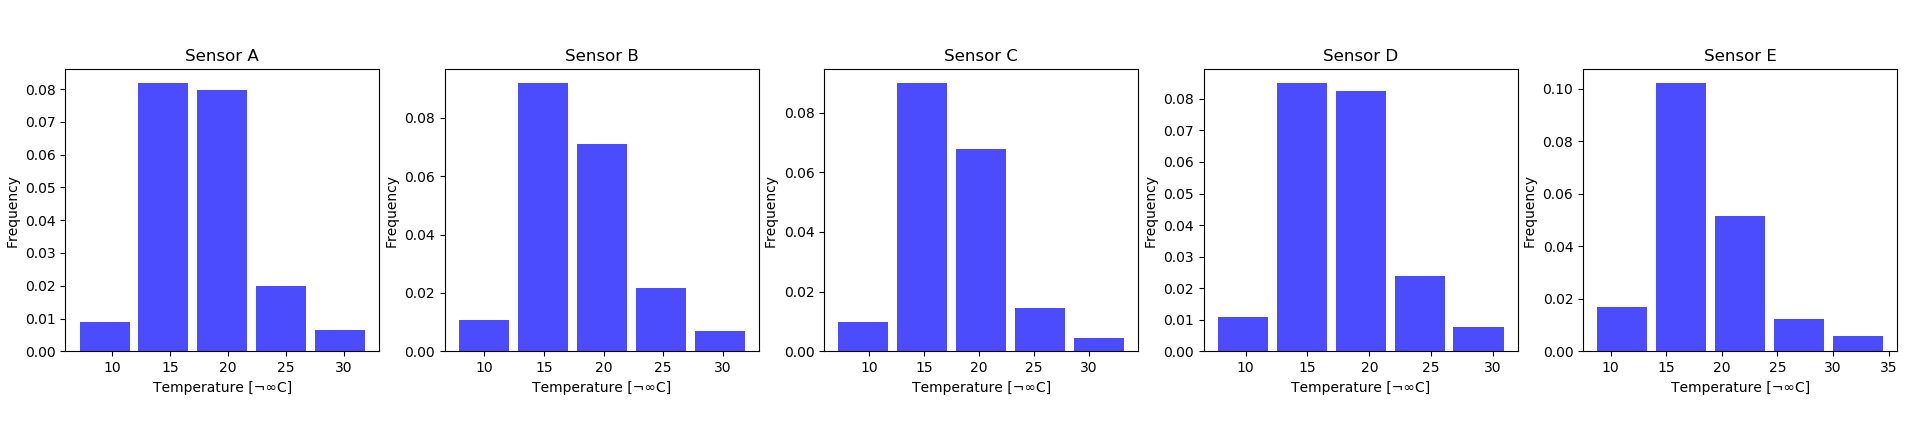
\includegraphics[width=\textwidth]{1-2-5_bins.png}
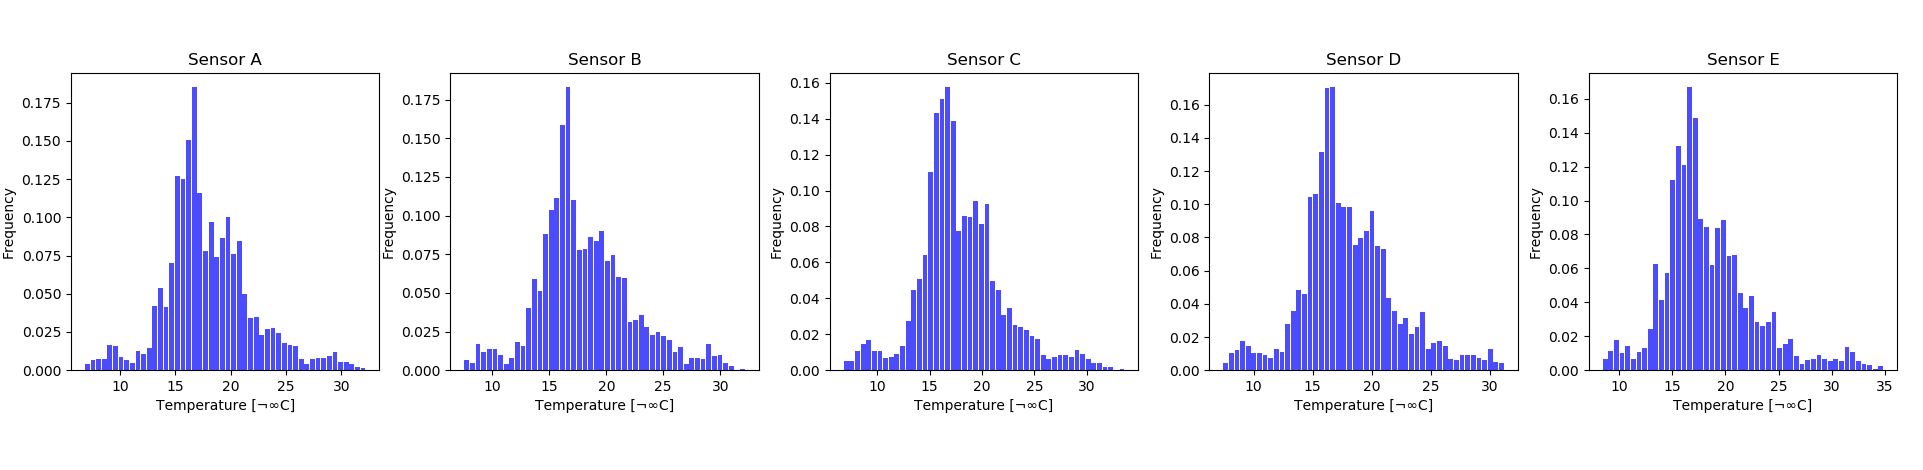
\includegraphics[width=\textwidth]{1-2-50_bins.png}
\caption{Comparison of different histogram binning settings}
\label{fig:1-2}
\end{figure}

\newpage

\subsection{Temperature Polygons}
\textit{
Create 1 plot where frequency polygons for the 5 sensors Temperature values overlap in different colors with a legend.
}\\

See Figure ~\ref{fig:1-3}.

\begin{figure}[!htb]
\centering
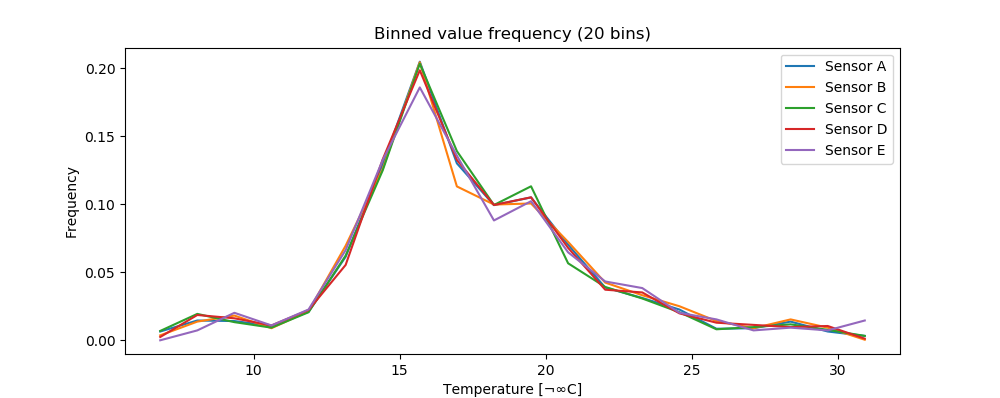
\includegraphics[width=\textwidth]{1-3-freq.png}
\caption{Temperature frequency polygons}
\label{fig:1-3}
\end{figure}

\subsection{Boxplots}
\textit{
Generate 3 plots that include the 5 sensors boxplot for: Wind Speed, Wind Direction and Temperature.
}\\

See Figure ~\ref{fig:1-4}

\begin{figure}[!htb]
\centering
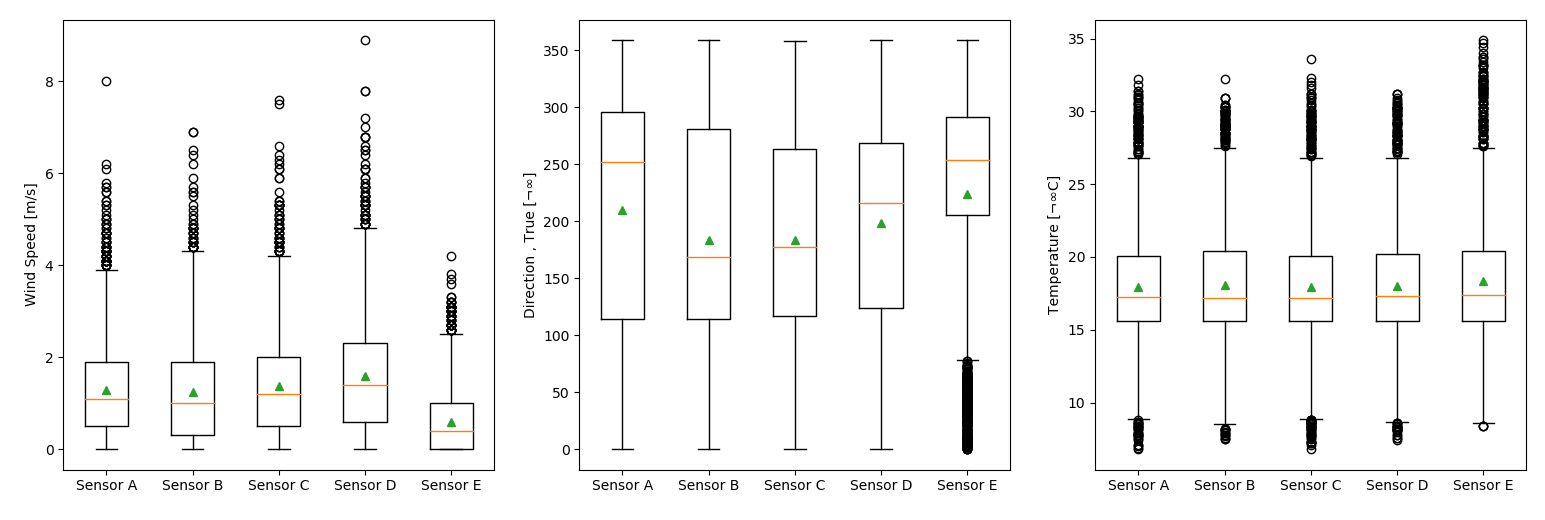
\includegraphics[width=\textwidth]{1-4-box.png}
\caption{Boxplots of Wind Speed, Direction and Temperature}
\label{fig:1-4}
\end{figure}


\section{Conclusion}
``I always thought something was fundamentally wrong with the universe''

\begin{figure}[ht!]
\centering
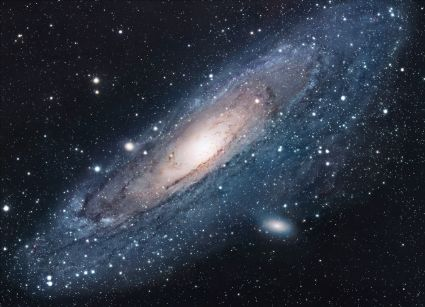
\includegraphics[scale=1.7]{universe}
\caption{The Universe}
\label{fig:universe}
\end{figure}

\bibliographystyle{plain}
\bibliography{references}
\end{document}
